\documentclass[12pt, notitlepage]{article}

\usepackage[utf8]{inputenc}
\usepackage{relsize}
\usepackage{authblk}
\usepackage{array}

\usepackage[table]{xcolor}
\usepackage{amssymb}
\usepackage{amsmath}
\usepackage{mathbbol}
\usepackage{bbm}
\usepackage{amsthm}
\usepackage{pdfpages}
\usepackage{graphicx,color,psfrag}
\usepackage{epstopdf}
\usepackage{pdflscape}
\usepackage{tabularx}
\usepackage{longtable}
\usepackage{breakurl}
\usepackage{enumitem}
\usepackage[normalem]{ulem}
\usepackage{blindtext}
\usepackage{fancyhdr}

\usepackage{newpxtext}

% caption fonts
\usepackage[font={large,bf}]{caption} 

\usepackage{setspace}
\usepackage{longtable}
\usepackage{threeparttable}  
\usepackage{tabulary}
\usepackage{booktabs}
\usepackage{float}
\usepackage{caption}
\usepackage{subcaption}
\usepackage{rotating}
\usepackage[titletoc,title]{appendix}

\usepackage{array,multirow}

\usepackage[round]{natbib}
\bibpunct{(}{)}{;}{a}{,}{;}
\setcounter{MaxMatrixCols}{10}

\topmargin=-1.8cm \textheight=23.8cm \oddsidemargin=-0.3cm
\evensidemargin=-0.5cm \textwidth=17.1cm
\newtheorem{ass}{Assumption}
\newtheorem{definit}{Definition}
\newtheorem{prop}{Proposition}
\newtheorem{cor}{Corollary}
\newtheorem{thm}{Theorem}
\newtheorem{lem}{Lemma}
\newtheorem{conj}{Conjecture}

\graphicspath{ {./images/} }

\usepackage{color}
\definecolor{myblue}{RGB}{0, 85, 165}
\usepackage[colorlinks=true,linkcolor=myblue, allcolors=myblue]{hyperref}
\usepackage{soul}

\pagestyle{fancy}
\fancyhf{}
\rhead{\textsc{Amedeus Akira Dsouza} \textsc{(}\textit{he}\textsc{/}\textit{him}\textsc{/}\textit{his}\textsc{)} \textsc{42975961}}
\lhead{\textsc{ECON 495 003}}

\cfoot{\thepage}

\title{\textsc{ECON 495 003: Paper Proposal}}
\author{\textsc{\href{https://sites.google.com/view/aadsouza}{Amedeus Akira Dsouza}}\thanks{Amedeus Akira Dsouza: \href{mailto:aa_dsouza@alumni.ubc.ca}{aa\_dsouza@alumni.ubc.ca}. We are extremely grateful to Nicole Fortin and Marit Rehavi for their continued guidance and support. We would like to thank Sheldon Birkett, Felipe Grosso, Elisabeth Hatting, Wenxin Ma, Javier Cort\'{e}s Orihuela, and Sarah Kirker Wappel for helpful discussions and comments.} \textsc{ (}\textit{he}\textsc{/}\textit{him}\textsc{/}\textit{his}\textsc{)} \textsc{42975961}\\\textsc{\href{https://economics.ubc.ca}{Vancouver School of Economics}, \href{https://www.ubc.ca}{University of British Columbia}}}
\date{\textsc{Wednesday, November 25, 2020}}

\begin{document}
\doublespacing
\maketitle
\thispagestyle{empty}
\begin{abstract}
We seek to understand the effect of labor market institutions - in particular, the minimum wage and labor unions - on racial earnings inequality along the earnings distribution, taking into account spillover effects. We expect to use an estimation strategy involving DFL decompositions, RIF regression analyses, and a difference-in-differences research design leveraging variation in state-level minimum wage increases. Therefore, we expect to contribute towards the literature on the disproportionate impacts of \textit{prima facie} race-neutral policies.
\end{abstract}
\clearpage
\pagenumbering{arabic}
\section{Introduction}
The broader question we seek to contribute towards answering is what is the effect of changes to labor market institutions on racial inequality. We expect to narrow this question down in multiple ways. First, we ask what are the effects of the decline of labor unions and changes to minimum wages on Black-white earnings inequality along the wage distribution taking into account spillover effects. We also ask how changes to the state-level minimum wage after 1970 affect the racial earnings gap.

We observe that emerging literature shines a spotlight on the efficacy of \textit{prima facie} race-neutral changes to labor market institutions on the outcomes of underrepresented workers \citep[see, for example,][]{derenoncourtmontialoux2020}. We note that this is not exclusive to labor markets. These analyses are a subset of the broader literature that looks at the disproportionate impacts of \textit{prima facie} race-neutral policies \citep[see, for example,][]{ahs2011}.  Strengthening labor market institutions -  by for example, increasing the minimum wage or encouraging and buttressing labor unions - could therefore potentially contribute towards reducing racial inequality. While targeted policies that seek to address these inequalities are indeed important, they are often limited in scope and susceptible to legal challenges.


\citet{derenoncourtmontialoux2020} shows us in \ref{fig1} the unadjusted Black-white earnings gap at the mean over time using data both from the CPS March Supplement and the decennial census. We clearly see that although the gap at the mean was reducing through the sixties and seventies, we start to have stagnation sometime around 1980 - and, if anything, we start to see a mild increase in the earnings gap at the turn of the twenty-first century. While the analysis put forth in \citet{derenoncourtmontialoux2020} zones in on the period of racial earnings convergence in the sixties and seventies, looking at the second panel of the plots in \ref{fig2} by \citet{barany2016}, we notice that periods of decrease in the real minimum wage may contribute towards the stagnation in the racial earnings gap after 1979. We note that \ref{fig1} only shows us the first moment which certainly does not characterize the whole earnings distribution. We see the non-uniformity of the distribution of the Black-white earnings gap smoothed for year fixed effects in \ref{fig3} by \citet{heywoodparent2012}. We observe the decline in private-sector unionization rates through the eighties and beyond as shown in \ref{fig4} but note the changing roles unions may have played over time and heterogeneity among unions at a given time with regards to racial inequality. We also note the consistent over-representation of Black people in private-sector unions.

We expect to use the cleaned CPS dataset from \citet{fll2019} as a starting point or to follow closely the cleaning procedure that gets the CPS May and MORG datasets to match \citet{fll2019}. We will closely follow the implementation of RIF on DFL in \citet{heywoodparent2012} who studied the effect of performance pay on racial inequality along the earnings distribution. We expect to manipulate the RIF regression following \citet{fll2019} to account for spillover effects. We will run a difference-in-differences regression leveraging state-level variation following \citet{cdlz2019} and \citet{derenoncourtmontialoux2020}. Our analysis would follow the same period as \citet{cdlz2019} but would look specifically at racial inequality, not just racial demographic heterogeneity. One possible extension we are exploring is using the finding in \citet{aganmakowsky2018} on the effect of minimum wage on recidivism to capture another spillover effect of the minimum wage on racial inequality. This would allow us to characterize the effect of the minimum wage more accurately given the significant number of Black men that are incarcerated and/or have criminal histories in the United States. 
\section{Literature Review}
The relationship between labor unions and racial wage inequality has long piqued cross disciplinary interest across the social sciences, including sociology \citep[see, for example,][]{rosenfeldkleykamp2012, mccall2001} and economics \citep[see, for example,][]{ashenfelter1972, boundfreeman1992}, and the racial aspect of unions and their members has been studied in the political sciences as well \citep[see, for example,][]{frymergrumbach2020}. We have noticed that it has been a while since this question has been thoroughly studied in published economics research. In this paper, we seek to revisit this relationship - we are interested in studying the effect of labor unions on the Black-white wage gap along the wage distribution taking into account spillover effects.

\citet{donohueheckman1991} explain that "the story of Black economic progress is not one of uniform secular advance, but rather of episodic change". Several policies and institutions have been evaluated for their potency and the mechanisms by which they reduce racial inequality, including the minimum wage \citep[see, for example,][]{derenoncourtmontialoux2020}, the Civil Rights Act of 1964 \citep[see, for example,][]{heckmanpayner1989, fgbh1973}, government transfer programs \citep[see, for example,][]{butlerheckman1977}. Factors that have been implicated as determinants of the Black-white gap include a focus on characteristics prior to labor market entry such as a skills gap \citep[see, for example,][]{nealjohnson1996}, parenting differences \citep[see, for example,][]{abhs2015}, and a college education \citep[see, for example,][]{abh2010}. The literature also alludes to under-representations of Black-white earnings inequality due to the growing absence of Black men in the workforce, in particular, due to incarceration \citep[see, for example][]{bayercharles2018, nealrick2014, chandra2003}. \citet{muellersmith2015} documents the persistent negative effects of incarceration on employment outcomes and on earnings. \citet{doleachansen2020} show that targeted policies such as "ban the box" - which sought to postpone questions about criminal history in order to reduce discrimination during hiring actually had unintended consequences where employers with a lack of information leaned into implicit biases. This is particularly relevant to our analysis due to the studied negative effect of the minimum wage on recidivism rates as shown by \citet{aganmakowsky2018}. We would like to make it very clear that we certainly do not suggest that all targeted policy interventions are unfruitful. \citet{miller2017} show that federal affirmative action programs had a significant effect on the percent of Black employees which persisted after the program was rendered moot.

A growing literature has sought to evaluate changes to labor market institutions and their effect on wage inequality \citep[see, for example,][]{clr2020, fll2019, fhkn2018, ams2016, ffl2009, dfl1996}. \citet{clr2020} document the contrasting decline of unionization in the private-sector and rise of unionization in the public sector. They explain that it thus follows that public sector unions have a larger effect on wage inequality. Using Gallup polling data going as far back as 1936, \citet{fhkn2018} show that unions indeed contributed to the fall in income inequality through the forties.

Looking beyond class-based perspectives, studies have also sought to approach inequality through demographic-specific analyses \citep[see, for example,][]{biasisarsons2020, blaukahn1996}. \citet{biasisarsons2020} look at the effect of flexible pay on the gender wage gap for teachers. In particular, they leverage the Wisconsin Budget Repair Bill (Act 10) that, among other things, placed severe limitations on the power of collective bargaining in public sector unions. \citet{biasisarsons2020} explain that as collective bargaining agreements expired, some school districts adopted a flexible pay model - including individual negotiations with teachers - which contributed to an increase in the gender wage gap. It is also possible that the presence of unions in the industry presents a barrier of hesitancy to firms with non-union workers seeking to adopt models such as flexible pay and performance pay.

\citet{ashenfelter1972} seeks to understand the effect of labor unions on racial discrimination in labor markets. He finds that on average racial discrimination is less prevalent in labor markets that are unionized but cautiously notes the presence of racial discrimination by labor unions themselves in the late sixties. This echoes the changing roles unions have played over time and the heterogeneity among unions in any given time as discussed by \citet{frymer2007} - from once being discriminatory and exclusionary, being indifferent about racial discrimination, to taking on leadership roles in the fight for civil rights. \citet{ashenfelter1972} also observes that the presence of labor unions had a positive effect on narrowing the Black-white wage gap over the same time period. \citet{leigh1978} is fascinated by the finding in \citet{ashenfelter1972} that craft unions - in contrast with industrial unions - had exacerbated the Black-white wage gap for men. \citet{leigh1978} also confirms said findings in \citet{ashenfelter1972} by looking at "middle-aged men". \citet{boundfreeman1992} explain that, among other factors, deunionization contributed to an increase in the Black-white wage gap among young men in the eighties. Our work is distinct from \citet{ashenfelter1972}, \citet{leigh1978}, \citet{boundfreeman1992} as we will be employing econometric tools that were developed after these papers were published and the focus of our discourse in the economics profession has shifted away from studying the effect of labor unions on racial inequality.

\citet{rosenfeldkleykamp2012} seek to understand the relationship between deunionization in the private-sector and racial wage inequality. Through counterfactual analysis, they find that deunionization contributes to exacerbating the Black-white wage gap - with the effect being stronger for women than for men. They explain that deunionization disproportionately affects Black workers as they are more likely to be in unions than white workers. They argue that the demand for protection against discrimination drives the over-representation of Black workers in unions. Similarly, they present that the difference between unionization for Black women relative to white women is greater than the difference for Black men relative to white men which explains the difference in the strength of the effect. Notably however, \citet{rosenfeldkleykamp2012} neither seem to account for spillover effects nor do they look at the effect of unions on racial wage inequality along the wage distribution. They compare the effects for union members to workers not in unions who would be "otherwise similar". This may be an issue in the presence of spillover effects - in particular union threat effects as discussed by \citet{fll2019}. As \citet{fll2019} explain, union threat effects capture the idea that firms may offer workers higher wages or higher benefits in order to placate interest in and threats to unionize. Looking at the overall distribution of racial inequality is indeed important as it allows us to specifically understand how these labor market institutions change the shape of the distribution and where in the distribution the effects are strongest. \citet{heywoodparent2012} notably find that the effect of performance pay through wage structure found in \citet{lmp2009} only applies to white people at the top end of the distribution.

Written effectively in response to \citet{ams2016}, \citet{fll2019} extend the analysis put forth in the seminal \citet{dfl1996} to include spillover effects when estimating the effect of the minimum wage on wage inequality and the effect of unions on the distribution of wages. \citet{ffl2009} develop the recentered influence function regression analysis and apply the method to understand the effects of labor unions on the unconditional wage dispersion accounting for both "within-group (same covariates)" and "between-group (different covariates)" effects.

\citet{bayercharles2018} document a decline in racial earnings inequality for men from 1940 to 1970 followed by an increase in racial earnings inequality at both the median and the 90th percentile when those with non-positive earnings are included in the analyses. They suggest, but do not test, that, among other factors, changing minimum wages and declining unionization contributes towards an effect on "distributional convergence" - "changes in the shape of the overall earnings distribution that affect Black–white relative earnings because [Black men] and [white men] occupy different initial positions in that distribution".

Our analysis indeed builds on the work put in by \citet{derenoncourtmontialoux2020} studying the effects of the minimum wage on racial inequality and is distinct in terms of the time period being studied, the better data available for the period being studied, the different dynamics of the racial earnings gap in the period being studied - in particular, the stagnation of the gap, and in the level of the policy changes being studied - federal vs. state-level changes to the minimum wage. We expect to further build on the topic in the coming weeks towards a more fruitful analysis in order to make a more significant contribution to the literature on labor market institutions and racial inequality.

\section{Data}
We shall use the Current Population Survey (CPS) Merged Outgoing Rotation Group as our primary dataset which is available from 1979 to 2019. In order to extend our analysis on labor unions, we shall extend our data using the CPS May back to 1973. We would like to consider supplementing our analysis with values imputed from the CPS Annual Social and Economic Supplement (ASEC). We expect our data to be the transpose of the following outline
\begin{center}
\footnotesize{
\begin{tabular}{|c|c|c|c|} 
\hline
Observation & 1 & ... & $n$\\
\hline
Survey Weight & & &\\
\hline
Survey Year & & &\\
\hline
Earnings & & &\\
\hline
Employment & & &\\
\hline
Benefits & & &\\
\hline
State Minimum Wage & & &\\
\hline
Union Coverage & & &\\
\hline
Race & & &\\
\hline
Ethnicity & & &\\
\hline
Sex & & &\\
\hline
State & & &\\
\hline
Urban & & &\\
\hline
Industry & & &\\
\hline
Age & & &\\
\hline
Marital Status & & &\\
\hline
Children & & &\\
\hline
Experience & & &\\
\hline
Education & & &\\
\hline
MSA & & &\\
\hline
\end{tabular}}
\end{center}
where
\begin{itemize}
    \item $n$ is the number of observations we have in our sample after cleaning the data.
    \item survey weight allows us to make inferences about the population using survey data.
    \item survey year records the year the survey was conducted.
\end{itemize}
We expect our dependent variables (Y variables) to be the following:
\begin{itemize}
    \item Earnings: Hourly wages (\$, CPS) consistent with \citet{fll2019}.
    \item Employment status (Dummy, CPS).
    \item Benefits - such as health insurance coverage (TBD, CPS).
\end{itemize}
We expect our independent variables (X variables) to be the following:
\begin{itemize}
    \item State minimum wage which we shall define as the maximum of the state minimum wage and the federal minimum wage unless state laws for specific states mandate otherwise. Several datasets for the same have been complied in the literature including Federal Reserve Economic Data from the Federal Reserve Bank of St. Louis found \hyperlink{https://fred.stlouisfed.org/tags/series?t=minimum+wage}{here}. We note that the Wages and Hour Division of the United States Department of Labor also maintains a database of changes to non-farm state-level minimum wages found \hyperlink{https://www.dol.gov/agencies/whd/state/minimum-wage/history}{here}. There also exists a dataset \hyperlink{https://equitablegrowth.org/working-papers/historical-state-and-sub-state-minimum-wage-data/}{here} that contributes towards the analysis put forth in \citet{derenoncourtmontialoux2020} We shall impute these values using the state and year variables found in the CPS.
    \item Union coverage (Dummy, CPS) consistent with \citet{fll2019}.
    \item Race (Dummy, CPS).
    \item Ethnicity (Dummy, CPS).
    \item Sex (Dummy, CPS).
\end{itemize}
Our covariates shall include:
\begin{itemize}
    \item Age (Integer, CPS).
    \item Marital Status (Dummy, CPS).
    \item Children (TBD, CPS).
    \item Education (TBD, CPS).
    \item Experience (TBD, CPS).
    \item MSA (TBD, CPS).
\end{itemize}
We note that \citet{chandra2003} identifies limitations in using CPS data - in particular, the presence of selection bias due to the exclusion of incarcerated people. Therefore, we should be cautious - and attempt to correct for this bias - as it implies that the CPS potentially understates racial inequality. 

We also intend on exploring in the coming weeks supplementing our analysis using the data from the decennial census and the American Community Survey (ACS) following \citet{bayercharles2018} which would allow for us to include these "non workers" in our analysis. Should this be possible, we could then incorporate the effect of the minimum wage on recidivism captured by \citet{aganmakowsky2018} using data from the National Corrections Reporting Program which we expect would increase the effect of the minimum wage on Black white earnings inequality.

\section{Estimation Strategy}
We break down our estimation strategy into to parts. First, we will follow the \citet{heywoodparent2012} implementation of the decomposition method developed by \citet{dfl1996} (here forth referred to as the DFL decomposition) and recentered influence function (RIF) regressions with spillover effects as found in \citet{fll2019}. Next, we shall leverage variation in state-level minimum wage increases to understand the effect of the minimum wage on the racial earnings gap after 1979 in a design similar to \citet{cdlz2019}.
\subsection{DFL Decomposition and RIF Regression}
\subsubsection{Labor Unions and Racial Earnings Inequality}
We want to understand what the earnings distribution for white people who are covered by a union would look like if they had the same covariates as Black people. Therefore if Black people and white people had the same education, experience, age, marital status, and children, were in the same states, in the same industries, all at the same time, what would the distribution for white people be? We expect to run these decompositions for the various permutations of race, ethnicity, and sex. We reiterate that the DFL and RIF regression we analyse closely follow the implementation in \citet{heywoodparent2012} and direct the reader to \citet{heywoodparent2012, fll2019, ffl2009, dfl1996} for a more thorough econometric review of the methods.

As shown in \citet{heywoodparent2012}, suppose the wage distribution for Black people $B = 1$ and white people $B = 0$ were given as
$$g(w\mid B = 1) = \int f(w\mid x, B = 1) h(x \mid B = 1) dx$$
$$g(w\mid B = 0) = \int f(w\mid x, B = 0) h(x \mid B = 0) dx.$$
Then, \citet{heywoodparent2012} show that the counterfactual wage distribution for white people if they had the same distribution of covariates as Black people is given by
$$g^c_{B = 1}(w\mid B = 0) = \int \Theta_1 f(w\mid x, B = 0) h(x\mid B = 0) dx$$
where $\Theta_1 =  \frac{Prob(B = 1\mid x) Prob(B = 0)}{Prob(B = 0\mid x)Prob(B = 1)}$.

Similarly, \citet{heywoodparent2012} show that the counterfactual wage distribution for white people in union jobs with the same distribution of covariates as Black people is given by
\begin{equation*}
g^c_{B=1, u = 1}(w\mid B = 0) = \int \Theta_2 f(w\mid x, B = 0, u = 1)h(x\mid B = 0, u = 1)dx
\end{equation*}
where $\Theta_2 = \frac{Prob(B = 1\mid x) Prob(u = 1\mid x, B = 1)}{Prob(B = 0\mid x)Prob(u = 1\mid x, B = 0)}$.

We note that this procedure is indeed similar to the Oaxaca-Blinder decomposition applied to the overall distribution, not just the mean. It allows us to find the effects that are explained by our covariates - what \citet{heywoodparent2012} call "composition effects", as well as the effects that remain unexplained.

Following \citet{heywoodparent2012}, we next seek to understand how our covariates influence these explained and unexplained effects. Therefore, for quantile $q(\tau)$, we have $RIF_i$ given by 
\begin{align*}
    RIF_i &= q(\tau) + \frac{\mathbbm{1}(w_i \geq q(\tau)) - (1-\tau)}{f(q(\tau))}\\
    &= \gamma_{1,\tau} \mathbbm{1}(w_i \geq q(\tau)) + \gamma_{2,\tau}
\end{align*}
where $\gamma_{1,\tau} = \frac{1}{f(q(\tau))}$ and $\gamma_{2,\tau} = q(\tau) - \gamma_{1,\tau} (1-\tau)$.
\citet{heywoodparent2012} run these RIF regressions for $q_{B = 0}(\tau)$, $q_{B = 1}(\tau)$, $q^C_{B = 1}(\tau)$ and parse $\Delta_\tau = q_{B = 0}(\tau) - q_{B=1}(\tau)$ as $$\Delta_\tau = [q_{B = 0}(\tau) - q^C_{B = 1}(\tau)] + [q^C_{B = 1}(\tau)- q_{B=1}(\tau)] = \Delta^X_\tau + \Delta^g_\tau.$$
We intend on following a similar procedure in our paper along with the extension in \citet{fll2019} to capture spillover effects. We are therefore able to move beyond the analysis of the first moment in \citet{rosenfeldkleykamp2012} to characterize the influence of labor unions along the earnings distribution on both the composition and the unexplained effects. We expect to implement the decomposition and RIF regression procedure to study the minimum wage after 1979 and racial inequality. For unions, as discussed in \citet{fll2019}, these spillover effects would include union threat effects. As \citet{fll2019} explain, firms may increase wages or increase access to benefits in order to placate any interest in organizing or potential unionization threat. For the minimum wage, \citet{fll2019} present that those weakly below the old minimum wage are not the only ones impacted by increases in the minimum wage as there may be "ripples" of an increase spilling over beyond the minimum. 
\subsection{State Minimum Wage Increases and Racial Earnings Inequality}
\citet{cdlz2019} note the presence of "138 prominent state-level minimum wage events, where states increased their minimum wage by at least \$0.25, and where at least 2\% of the workers were directly affected by the increase" over the time period they study - 1979 to 2016. Therefore we expect to run the following regression
\begin{multline*}
   \ln(w_{ijst}) = \sum_{\tau = -3}^{4}\alpha_\tau (Treat_{st}^\tau \times Black_i) +\theta_\tau Treat_{st}^\tau+ \beta Black_i +
   \zeta_j + \lambda_s +  \delta_t + X'_{ijst}\Gamma + \epsilon_{ijst},
\end{multline*}
where $\ln(w_{ijst})$ are log earnings of worker $i$ in industry, state, and at time $jst$ respectively. Notice that $Treat_{st}^\tau$ tells us if the treatment, that is, the minimum wage increase takes place $\tau$ periods from time $t$ in state $s$. $Black_i$ tells us if individual $i$ is a Black person. Notice as well that, $\zeta_j$, $\lambda_s$, $\delta_t$ are industry, state, and time fixed effects respectively. $X_{ijst}$ captures the covariates we include in our model including the smaller state-level and all federal level minimum wage policy changes \citep[see,][]{cdlz2019}. These include controls for union status, education, experience, squared experience, age, squared age, sex, marital status, children, ethnicity, occupation, and number of hours worked - similar to \citet{derenoncourtmontialoux2020}. We see then that $\alpha_\tau$ is our coefficient of interest which captures the effect of the state-level increase in the minimum wage for Black people in the years preceding and proceeding the treatment. We expect our findings to be consistent with \citet{derenoncourtmontialoux2020} who found that an increase in the federal minimum wage in 1967 significantly contributed to the fall in racial earnings inequality.
Consistent with \citet{cdlz2019} and \citet{derenoncourtmontialoux2020}, we expect to cluster our standard errors at the state-level.

We also intend to run a quantile regression at the $90-10$ and $50-10$ differentials to get a better understanding about where the effects are the strongest. As does \citet{cdlz2019}, we would like to make use of the Kaitz index which is the minimum wage to median wage ratio in our analysis.

As this is a difference-in-differences analysis, in addition to our ordinary least squares Gauss-Markov assumptions, we would need to ensure that common trends and excludability are satisfied. For the common trends assumption we would need that the racial earnings gap would not have changed without our treatment. For excludability, we need to ensure that there were no concurrent events affecting the racial earnings gap alongside increases to the state-level minimum wage. We are reassured by the fact that we are leveraging over a hundred policy interventions as we would need to find concurrent events that systematically bias our results in a particular direction. We intend on putting our estimates through a barrage of falsification tests. In particular, we can test arbitrary pre-treatment state-times to check if we find no effects on the racial earnings gap.

We could also look at sub-samples where we expect the effect to be stronger - in particular youth employment. We also expect our results to be robust to controls being added to and taken away from the model. As does \citet{cdlz2019}, we could break down our analysis and run our regressions in order to test each of the individual policy changes. We explored the idea of testing people in the upper end of the distribution as a relevant subsample where we had believed it to be reasonable to not find any spillover effects. However, we learned about the findings in \citet{barany2016} who showed that increases in the minimum wage affect decisions about human capital accumulation which would significantly effect those at the upper end of the distribution. In order to enrich our analysis we indeed intending at exploring heterogeneity by demographic groups including age, sex, and ethnicity.

With our analysis on unions, we are concerned about omitted variables including the composition of unions themselves. \citet{frymergrumbach2020} note that "white union members have lower racial resentment and greater support for policies that benefit [Black people]". Therefore, it is possible that effects we find may not be driven by the institution of unions, collective bargaining, and organizing itself, but from a collection of like-minded people that are cognizant about racial biases and discrimination. \citet{brown1984} documents that "censoring" workers who earn neither a wage nor a salary - that is those who have "dropped out" of the labor market - in published median earnings leads to an underestimation of the Black-white wage gap and suggests corrections to estimates.

\section{To-Do List}
Please note that our list takes the format: Task - Approximate Duration - Anticipated Completion Date.
\begin{itemize}
    \item Create GitHub repository for version control - 1 day - November 30, 2020.
    \item Complete THOROUGH review of minimum wage literature and racial inequality literature; build literature annotation table - 1 month - December 22, 2020.
    \item Pin down major changes to independent and dependent variables and focus analysis - 2 weeks - December 18, 2020.
    \item Adjust and enrich analysis building off \citet{derenoncourtmontialoux2020} - 1 month - December 22, 2020.
    \item Holiday break for mental health - 1 week - December 31, 2020.
    \item Practice running DFL and RIF regressions using assignments from ECON 561 - 1.5 weeks - December 31, 2020.
    \item Download and clean CPS May and MORG datasets (if possible using cleaned data from \citet{fll2019} which would reduce duration to 1 week) - 3 weeks - January 10, 2021.
    \item Load and merge supplementary datasets including minimum wage data, census data, ACS data, ASEC data as necessary - 3 weeks - January 20, 2021.
    \item Prepare document with summary statistics - 1 week - January 25, 2021.
    \item Pin down regression equations to be run - 2 weeks - Feb 14, 2021.
    \item DFL and RIF analysis with necessary adjustments - 3 weeks - Feb 20, 2021.
    \item State minimum wage regression analysis with necessary adjustments - 1 month - March 6 2021.
    \item Robustness checks, falsification tests, subsampling, adding controls to model - 2 weeks, March 10, 2021.
    \item Writing rough draft of thesis - 1 month - March 24, 2021.
    \item Develop and implement palette and template for consistent plots - 1 week - April 3, 2021.
    \item Final edits on thesis - 1.5 weeks - April 5, 2021. (4 day buffer to submission)
    \item Thesis revision - 2 weeks - April 30, 2021.
\end{itemize}

\singlespacing
\pagebreak
\bibliographystyle{apalike}
\nocite{*}
%citation rules 
%\citet{foo} outside 
%\citep[see, for example,][]{foo}
%no \citex*{}
%in bib: two authors fortinlemieuxXXXX; three authors dflXXXX.

{\footnotesize\bibliography{495preliminaryprospectus}}

\pagebreak
\appendix
\section{Figures}
\subsection{Figure 1 - Black-white Earnings Gap at Mean - \citet{derenoncourtmontialoux2020}}\label{fig1}
\begin{figure}[h!]
\centering
    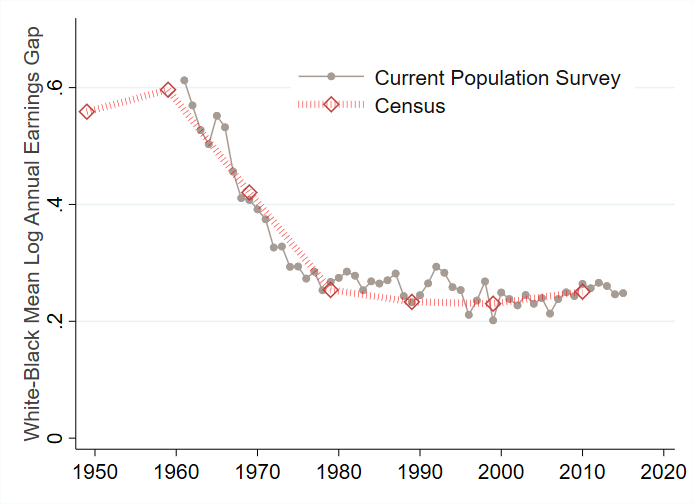
\includegraphics[width=\textwidth, height = 0.8\textheight, keepaspectratio]{unadj_rg_all_1949_2017.png}
\end{figure}
\pagebreak
\subsection{Figure 2 (panel 2) - Real Federal Minimum Wage over Time in 2000 \$ - \citet{barany2016}}\label{fig2}
\begin{figure}[h!]
\centering
    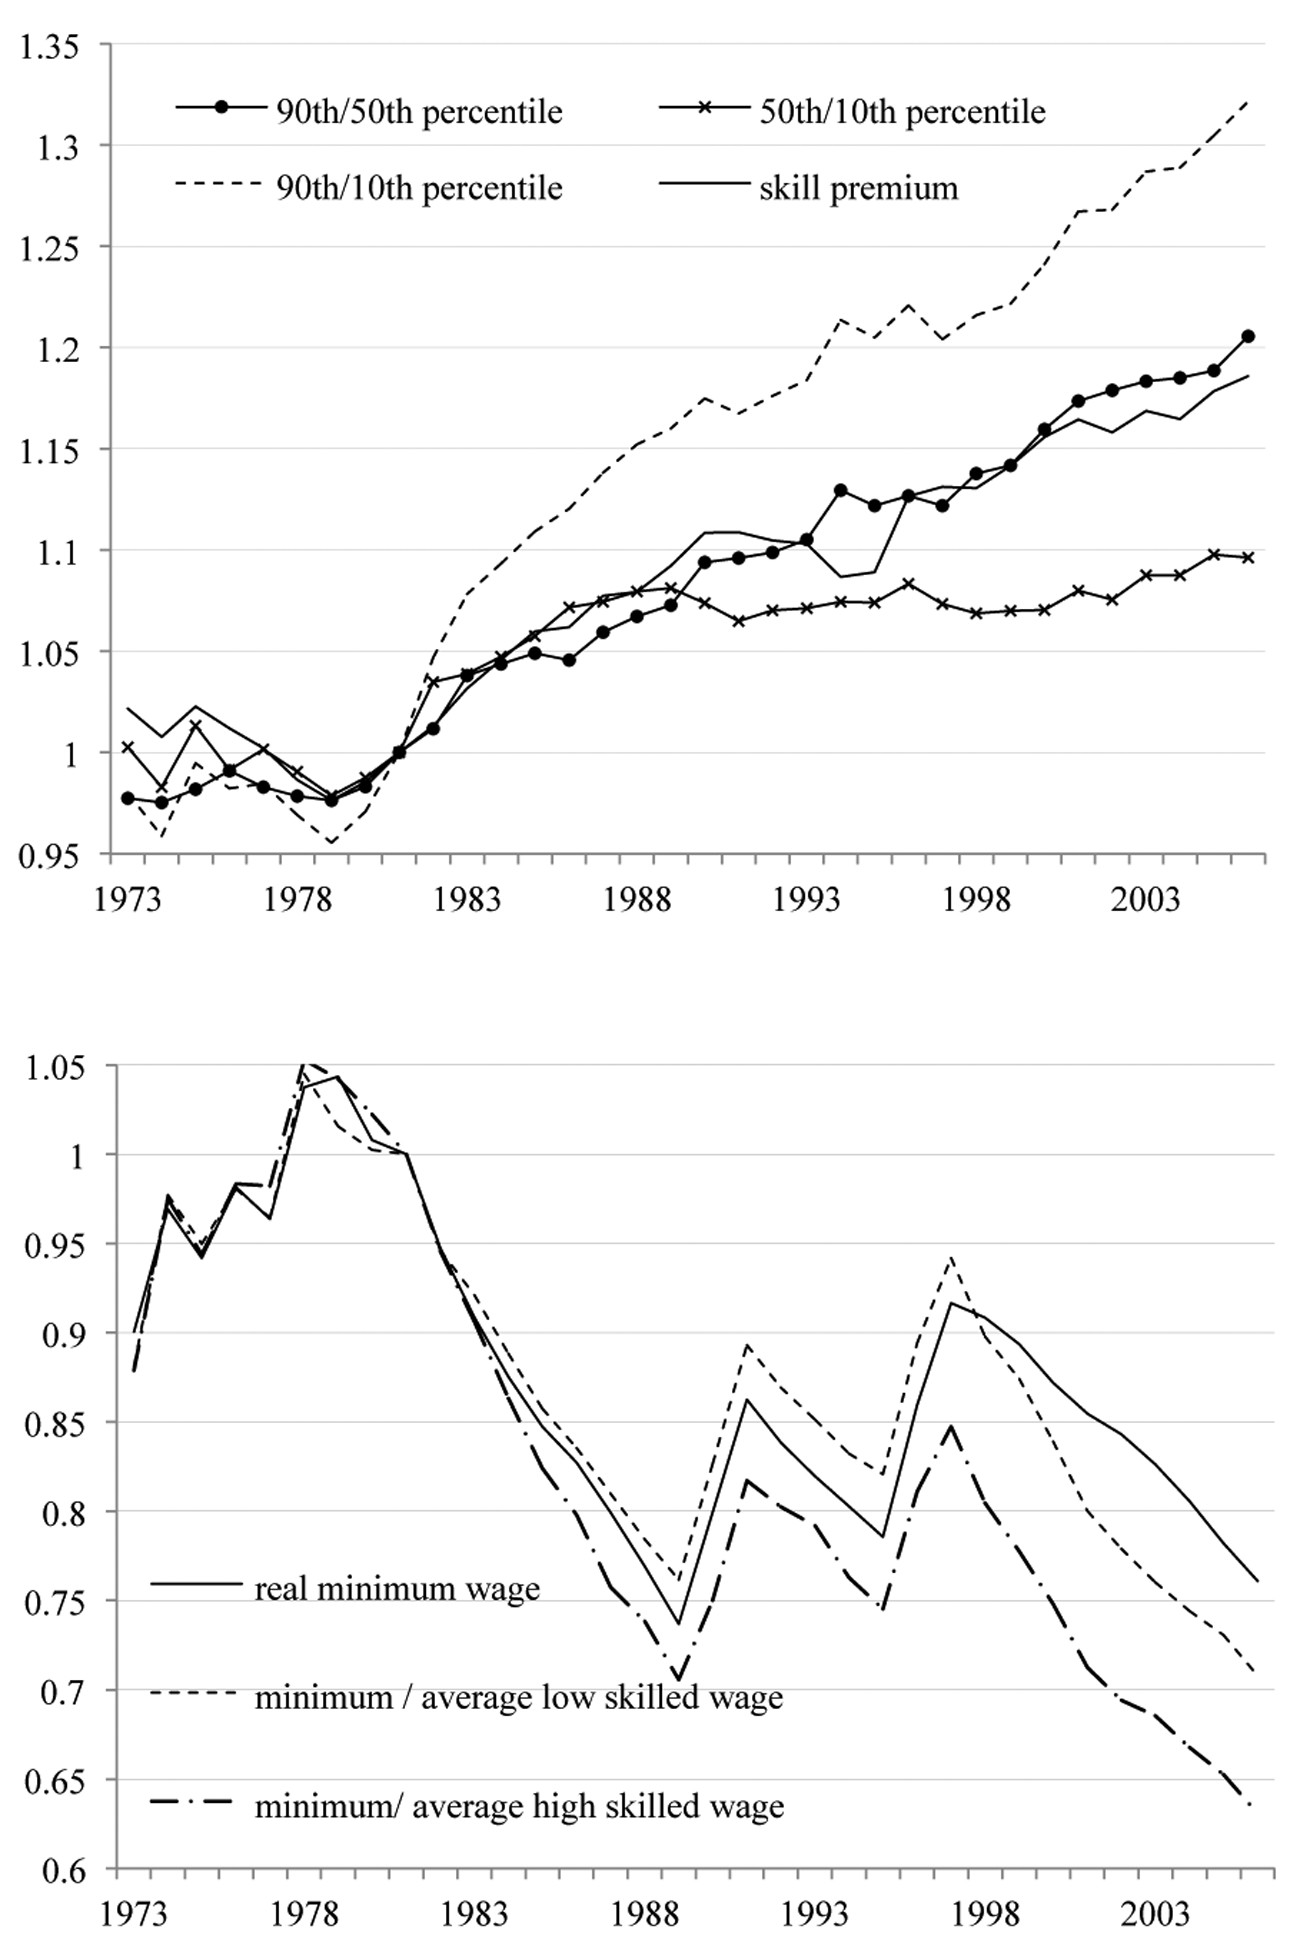
\includegraphics[width=\textwidth, height = 0.8\textheight, keepaspectratio]{barany.jpeg}
\end{figure}
\pagebreak
\subsection{Figure 3 - Black-white Earnings Gap Distribution - \citet{heywoodparent2012}}\label{fig3}
\begin{figure}[h!]
\centering
    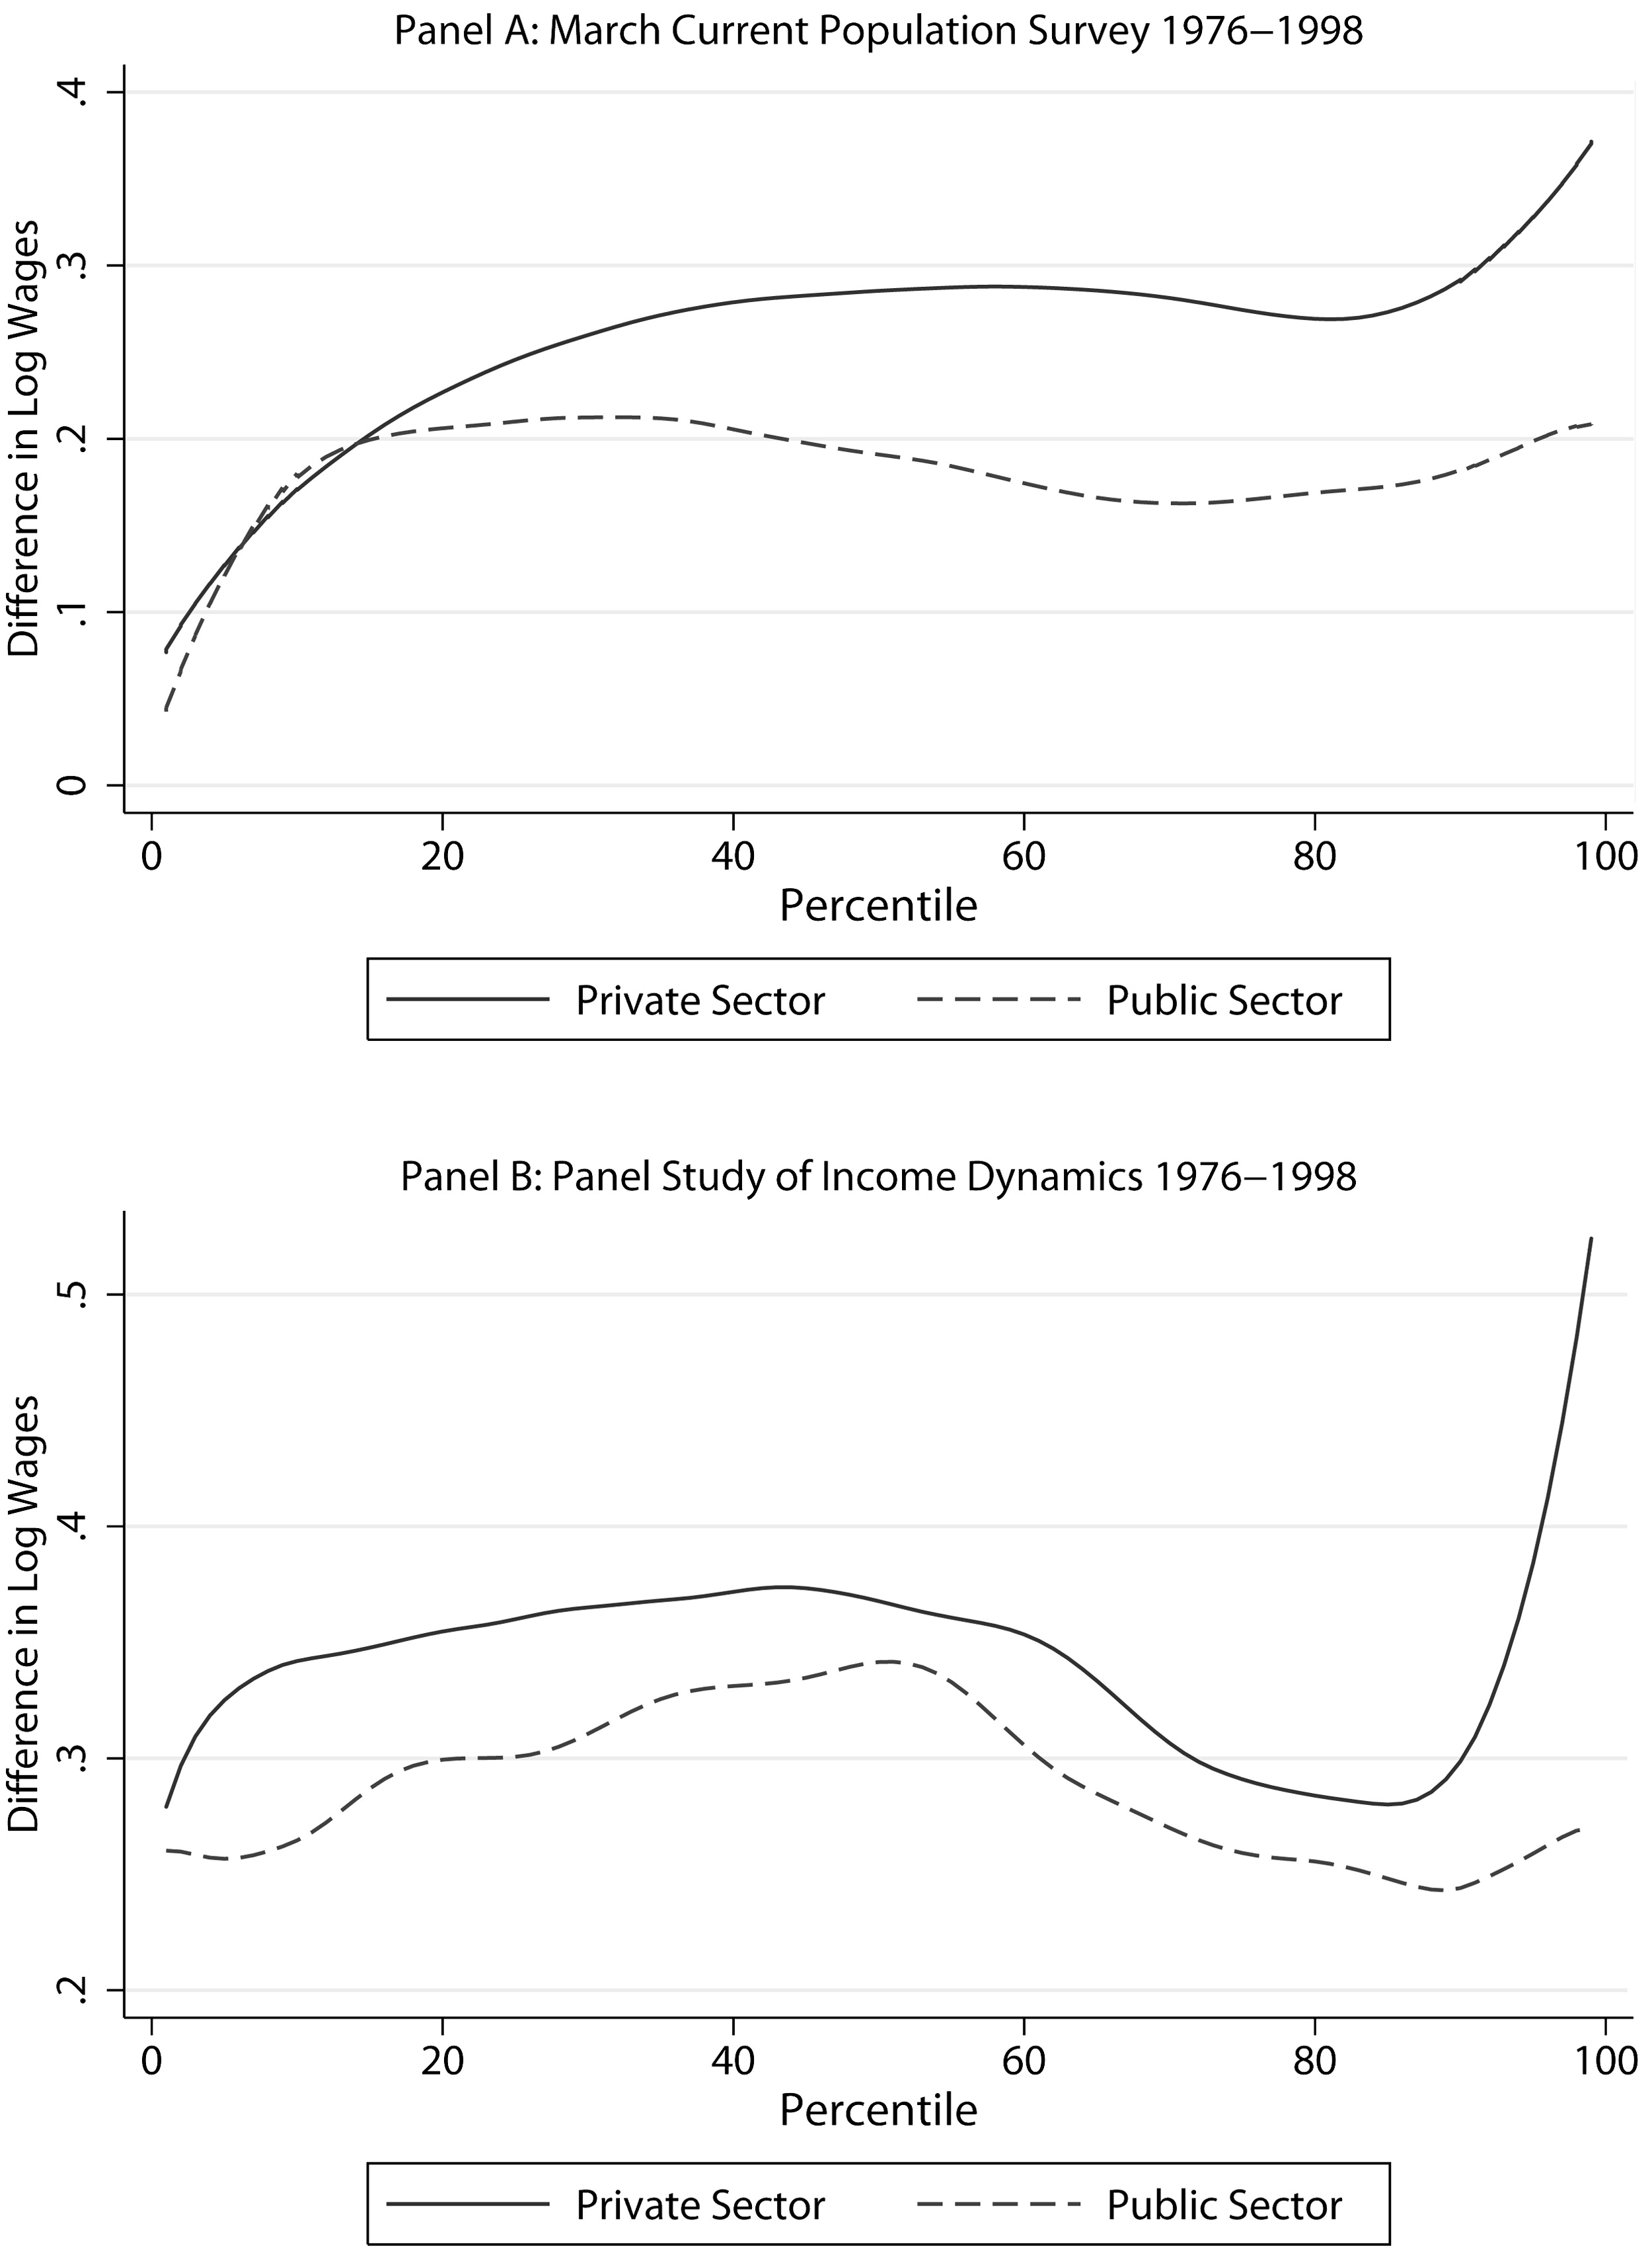
\includegraphics[width=\textwidth, height = 0.8\textheight, keepaspectratio]{fg1.jpg}
\end{figure}
\pagebreak
\subsection{Figure 4 - Union Membership by Race - \citet{rosenfeldkleykamp2012}}\label{fig4}
\begin{figure}[h!]
\centering
    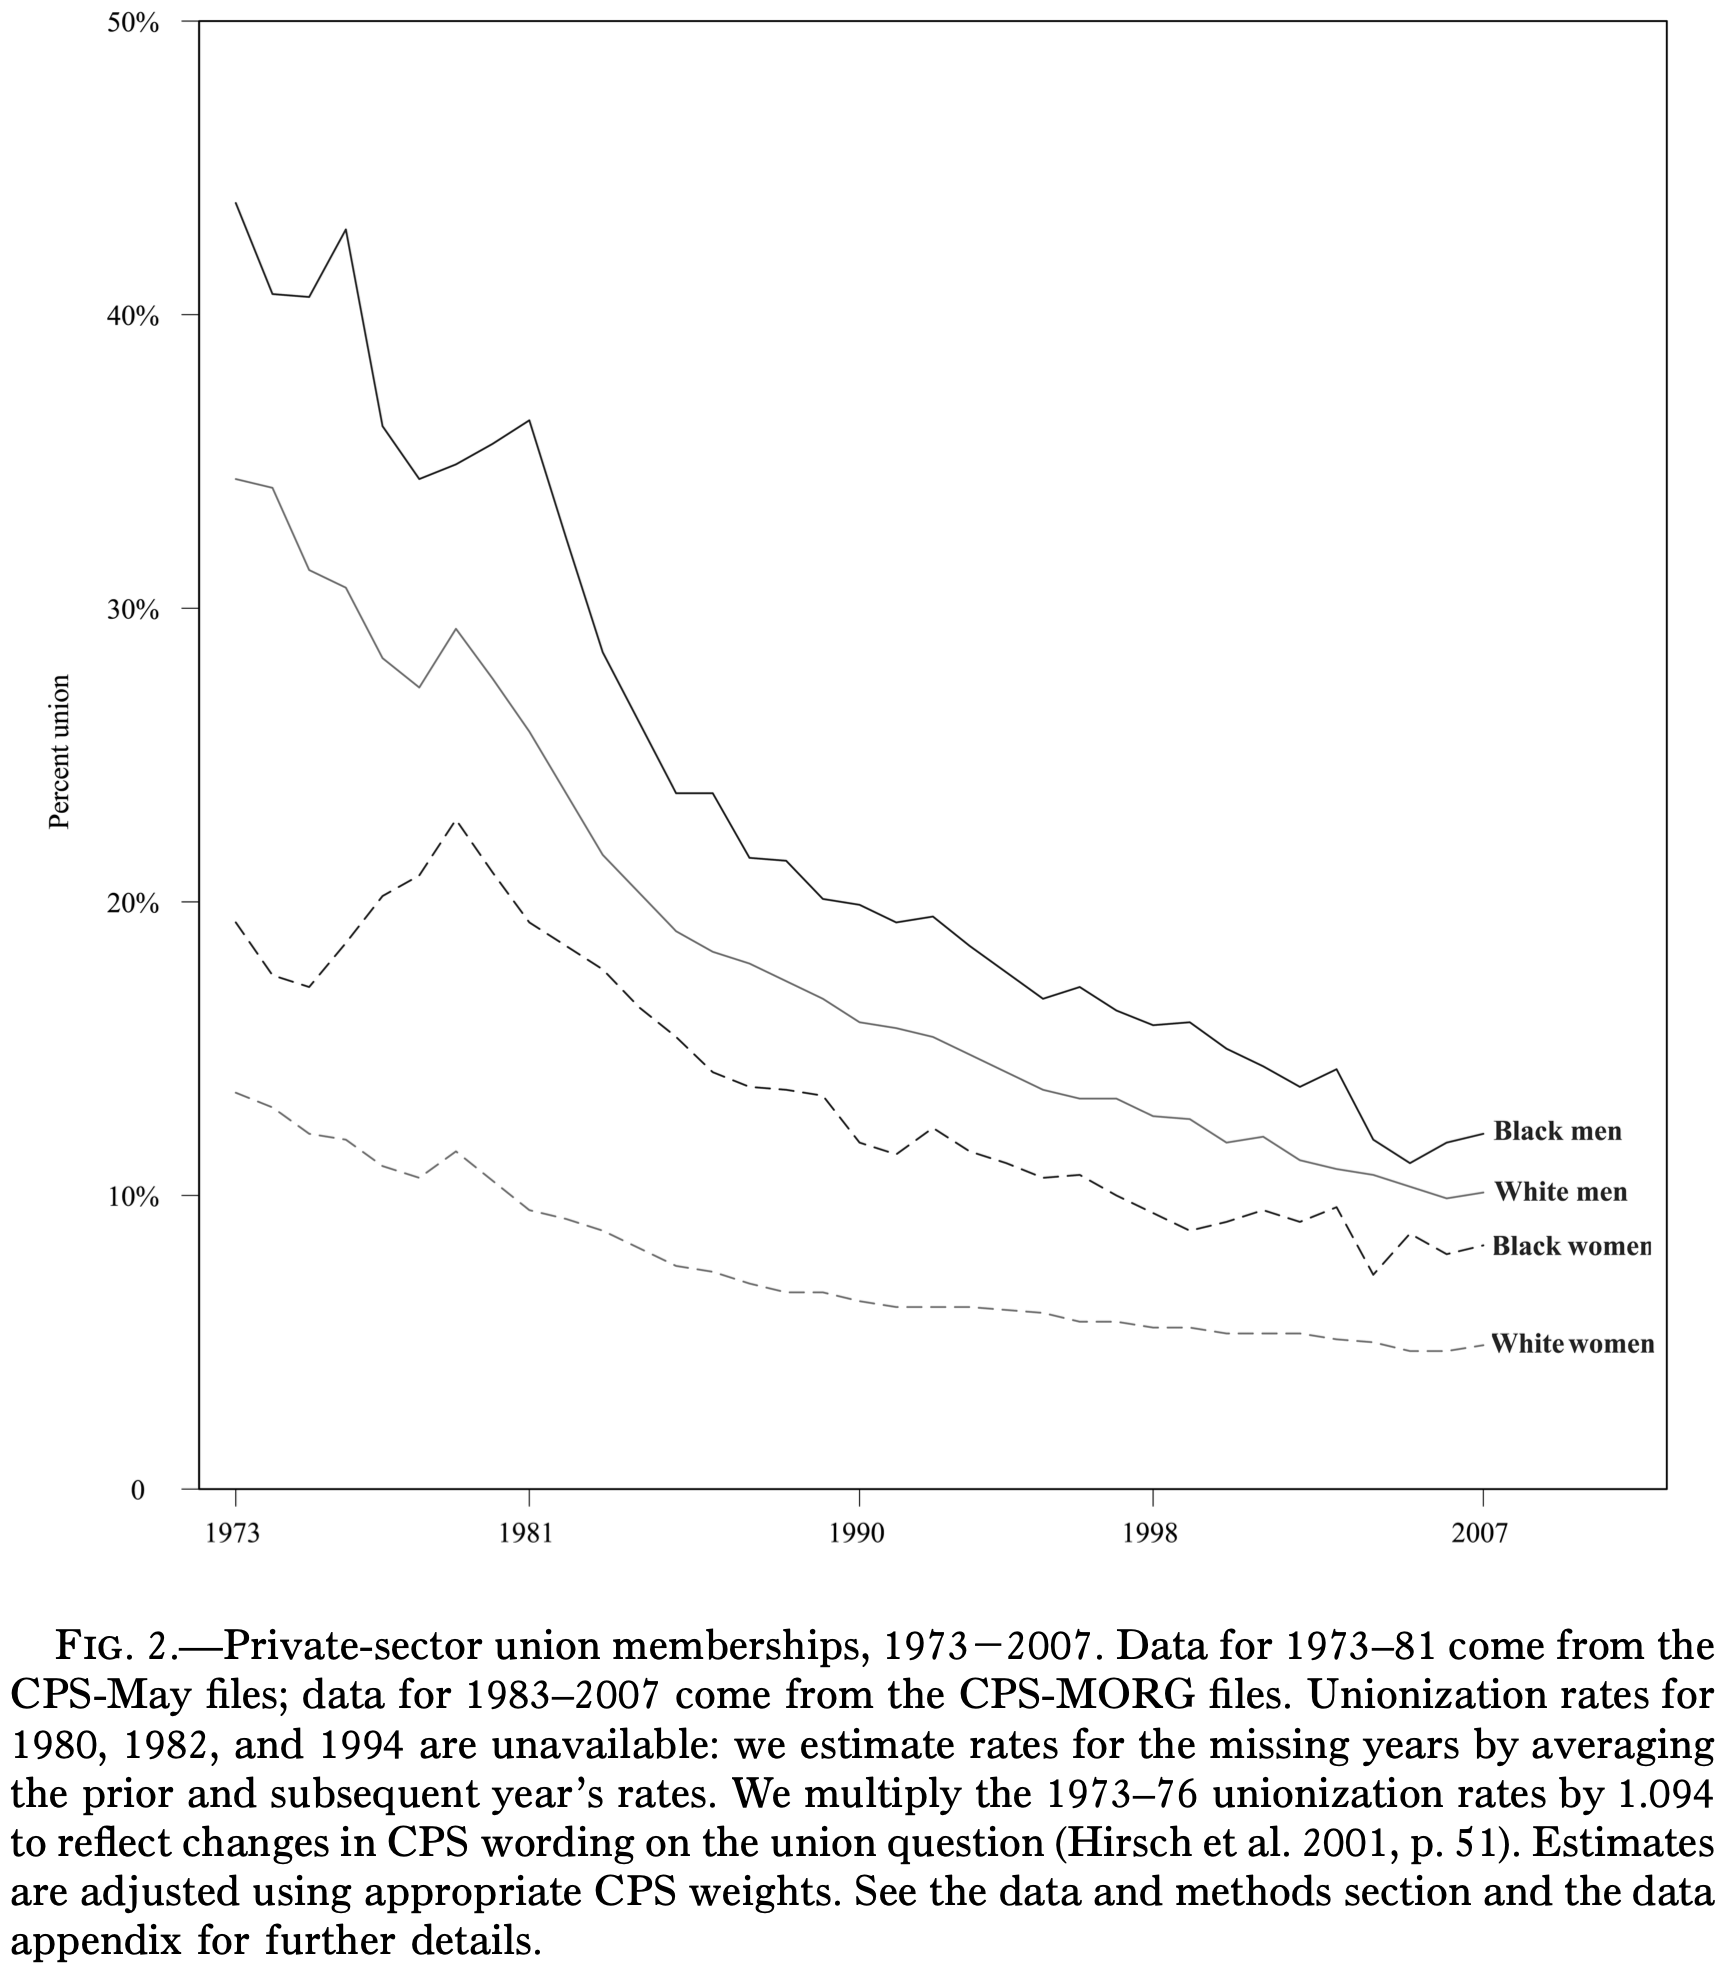
\includegraphics[width=\textwidth, height = 0.8\textheight, keepaspectratio]{rk_fig2.png}
\end{figure}
\end{document}


